\documentclass[12pt,a4paper]{article}

\usepackage[a4paper,text={16.5cm,25.2cm},centering]{geometry}
\usepackage{lmodern}
\usepackage{amssymb,amsmath}
\usepackage{bm}
\usepackage{graphicx}
\usepackage{microtype}
\usepackage{hyperref}
\usepackage{minted}
\setlength{\parindent}{0pt}
\setlength{\parskip}{1.2ex}

\hypersetup
       {   pdfauthor = {  },
           pdftitle={  },
           colorlinks=TRUE,
           linkcolor=black,
           citecolor=blue,
           urlcolor=blue
       }






\begin{document}



\section{Nelinearne enačbe}
Iščemo rešitev nelinearne enačbe $f(t) = F(x(t),y(t),z(t)) = 0$, kjer je t spremenljivka. Uporabimo Newtonovo metodo.


Poiščemo presečišče $y = sin(x)$ in $y = cos(x)$


\begin{minted}[texcomments = true, mathescape, fontsize=\small, xleftmargin=0.5em]{julia}
using Vaje07
using Plots
using ForwardDiff
f(x) = sin(x) - cos(x)
df(x) = cos(x) + sin(x)
x, it = newton(f,df,0.0)

plot(sin,0,2*|$\ensuremath{\pi}$|)
plot!(cos,0,2*|$\ensuremath{\pi}$|)
scatter!([x],[sin(x)])
\end{minted}
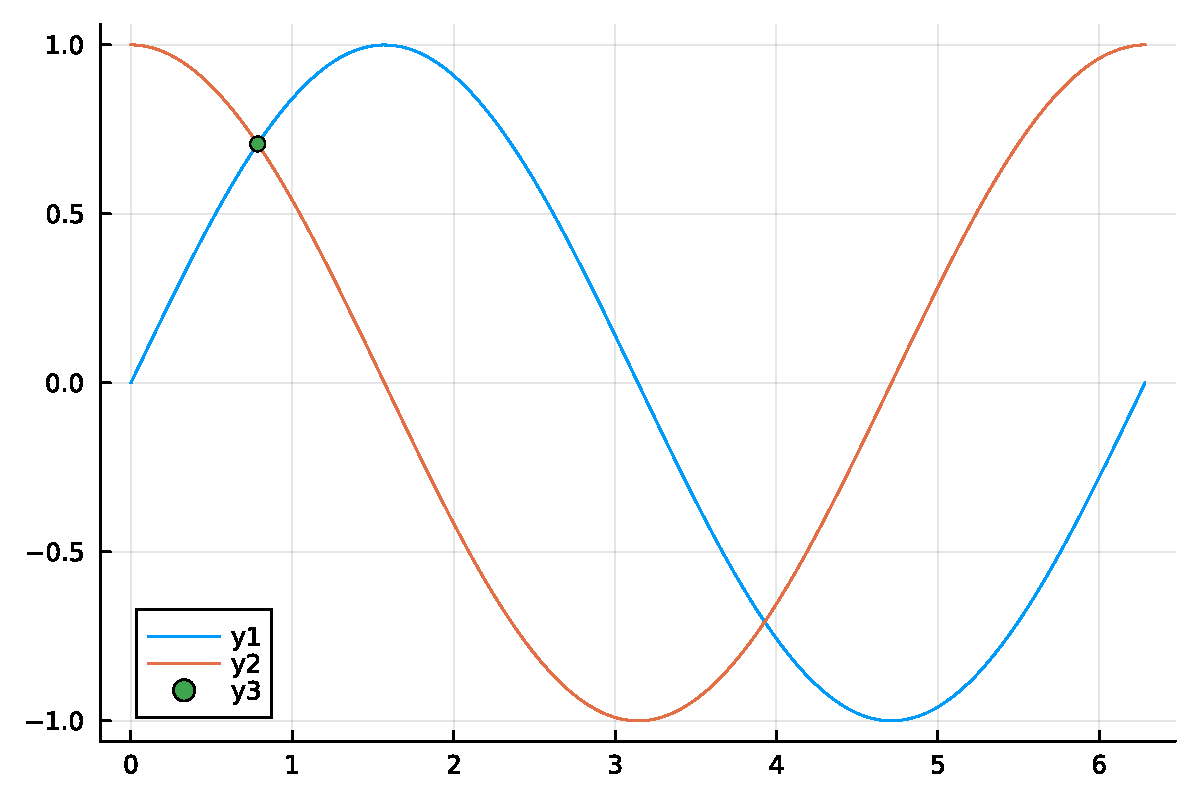
\includegraphics[width=\linewidth]{jl_UT2mFa/demo_1_1.pdf}

Poiščemo presečišče med poltraka in ploskve


\begin{minted}[texcomments = true, mathescape, fontsize=\small, xleftmargin=0.5em]{julia}
x0 = [0,0,0] # Začetna točka poltraka
e = [1,1,0.1] # Smerni vektor poltraka
r = 2
R = 3
F(x) = (R - sqrt(x[1]^2 + x[2]^2))^2 + x[3]^2 - r # Enačba torusa
DF(x) = 2 * vcat((-R/sqrt(x[1]^2 + x[2]^2) - 1) .* x[1:2],x[3])
autoDF(x) = ForwardDiff.gradient(F,x)
p = presecisce((x0,e), F,DF, 1.0)
\end{minted}
\begin{minted}[texcomments = true, mathescape, fontsize=\small, xleftmargin=0.5em, frame = leftline]{text}
3-element Vector{Float64}:
 1.1244865308096843
 1.1244865308096843
 0.11244865308096844
\end{minted}

spremenljivka


\begin{minted}[texcomments = true, mathescape, fontsize=\small, xleftmargin=0.5em]{julia}
function z(x,y) 
    z2 = r^2 - (R - sqrt(x^2 + y^2))^2
    if z2 < 0
        return 0
    else
        return sqrt(z2)
    end
end
x = LinRange(-5,5,100)
y = LinRange(0,5,100)
surface(x,y,z)

plot!([x0[1],p[1]],[x0[2],p[2]],[x0[3],p[3]])
\end{minted}
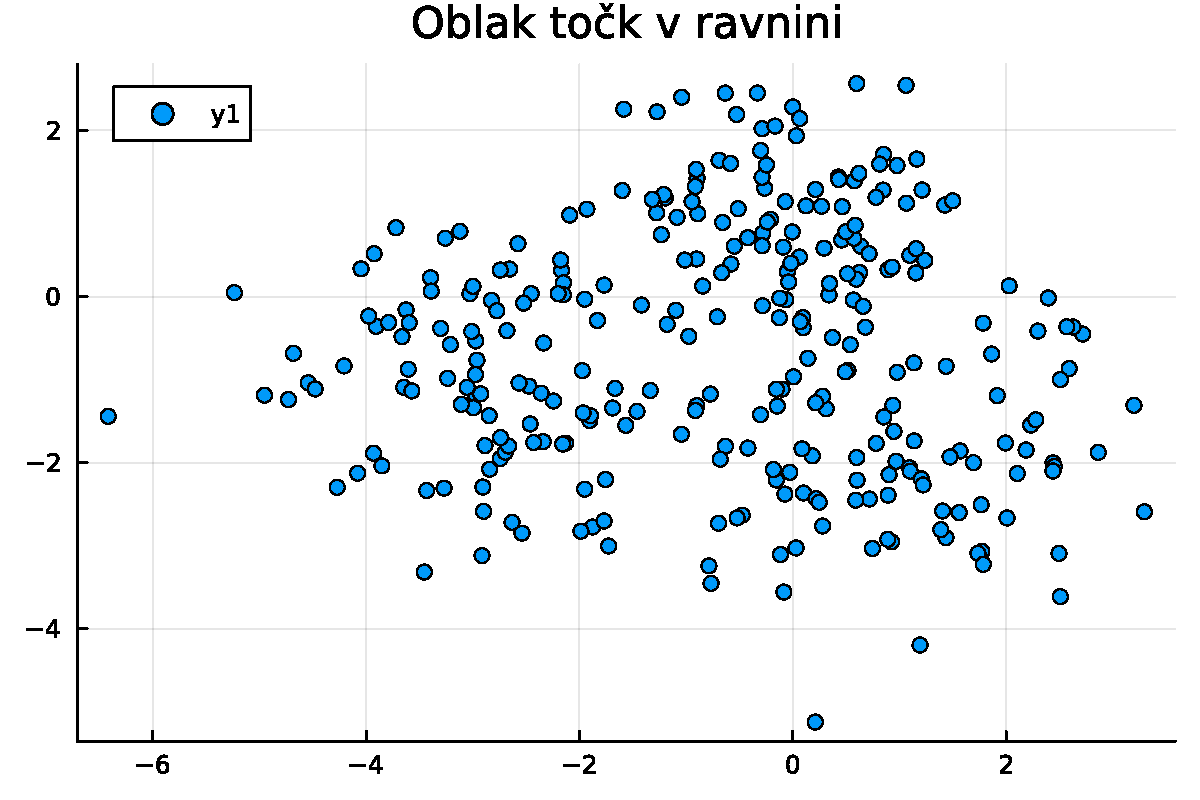
\includegraphics[width=\linewidth]{jl_UT2mFa/demo_2_1.pdf}


\end{document}
